\subsection{Revis\~ao sistem\'atica da literatura} \label{subsec:revisão}

As séries temporais desempenham um papel fundamental em diversos campos do conhecimento, como Economia (preços diários de estoques, taxa de desemprego mensal, produção industrial), Medicina (eletrocardiograma, eletroencefalograma), Epidemiologia (número mensal de novos casos de meningite), Meteorologia (chuvas, temperatura diária, velocidade do vento), entre outros. Ao longo dos anos, têm sido empregadas ferramentas computacionais para tornar a previsão em séries temporais mais eficiente, especialmente com o uso de técnicas de aprendizado de máquina e linguagens de programação como \textit{Python} e \textit{R}, que se destacam por sua capacidade de manipular e analisar dados temporais de forma eficaz.

Para compreender melhor o conceito de série temporal, é possível considerar o exemplo de um maratonista que pratica corrida regularmente ao longo de vários anos e uma pessoa sedentária que decide participar de uma corrida com uma distância máxima de 5 km. Ambos realizam a corrida ao mesmo tempo, utilizando monitores de frequência cardíaca que permitem o acompanhamento médico. Ao analisar os dados desde o início até o final da corrida, é possível observar que a série temporal do maratonista apresenta um comportamento mais estacionário, devido ao seu hábito regular de corrida. Por outro lado, a série temporal da pessoa sedentária é mais não estacionária, como ilustrado na Figura \ref{fig:series}. Essa diferença ocorre devido à falta de regularidade na prática de exercícios físicos por parte da pessoa sedentária.

\begin{figure}[H]
	\centering
	\caption{Exemplo de séries temporais}
	\label{fig:series}
	\includegraphics[width=0.9\linewidth]{Revisao/Figuras/séries}
	
	Fonte: \cite{brandão_2020}
\end{figure}


Na Figura \ref{fig:series}, é possível observar que o eixo $x$ representa os dados observados ao longo do tempo, enquanto o eixo $t$ representa o tempo decorrido. Além disso, as séries temporais são caracterizadas como processos estocásticos regidos por leis probabilísticas. Isso implica que elas podem ser concebidas como um conjunto de todas as possíveis trajetórias que uma variável alvo pode seguir, como ilustrado na Figura \ref{fig:series}. No entanto, somente uma dessas trajetórias será observada, de acordo com as características que se manifestaram durante o período analisado. Por exemplo, ao lançar um dado, existem seis possibilidades, mas apenas um número será obtido. Da mesma forma, em séries temporais, há uma infinidade de possibilidades, mas somente uma delas ocorrerá, de acordo com as características que se apresentaram nesse determinado período.

\begin{figure}[H]
	\centering
	\caption{Processo estocástico}
	\label{fig:serie}
	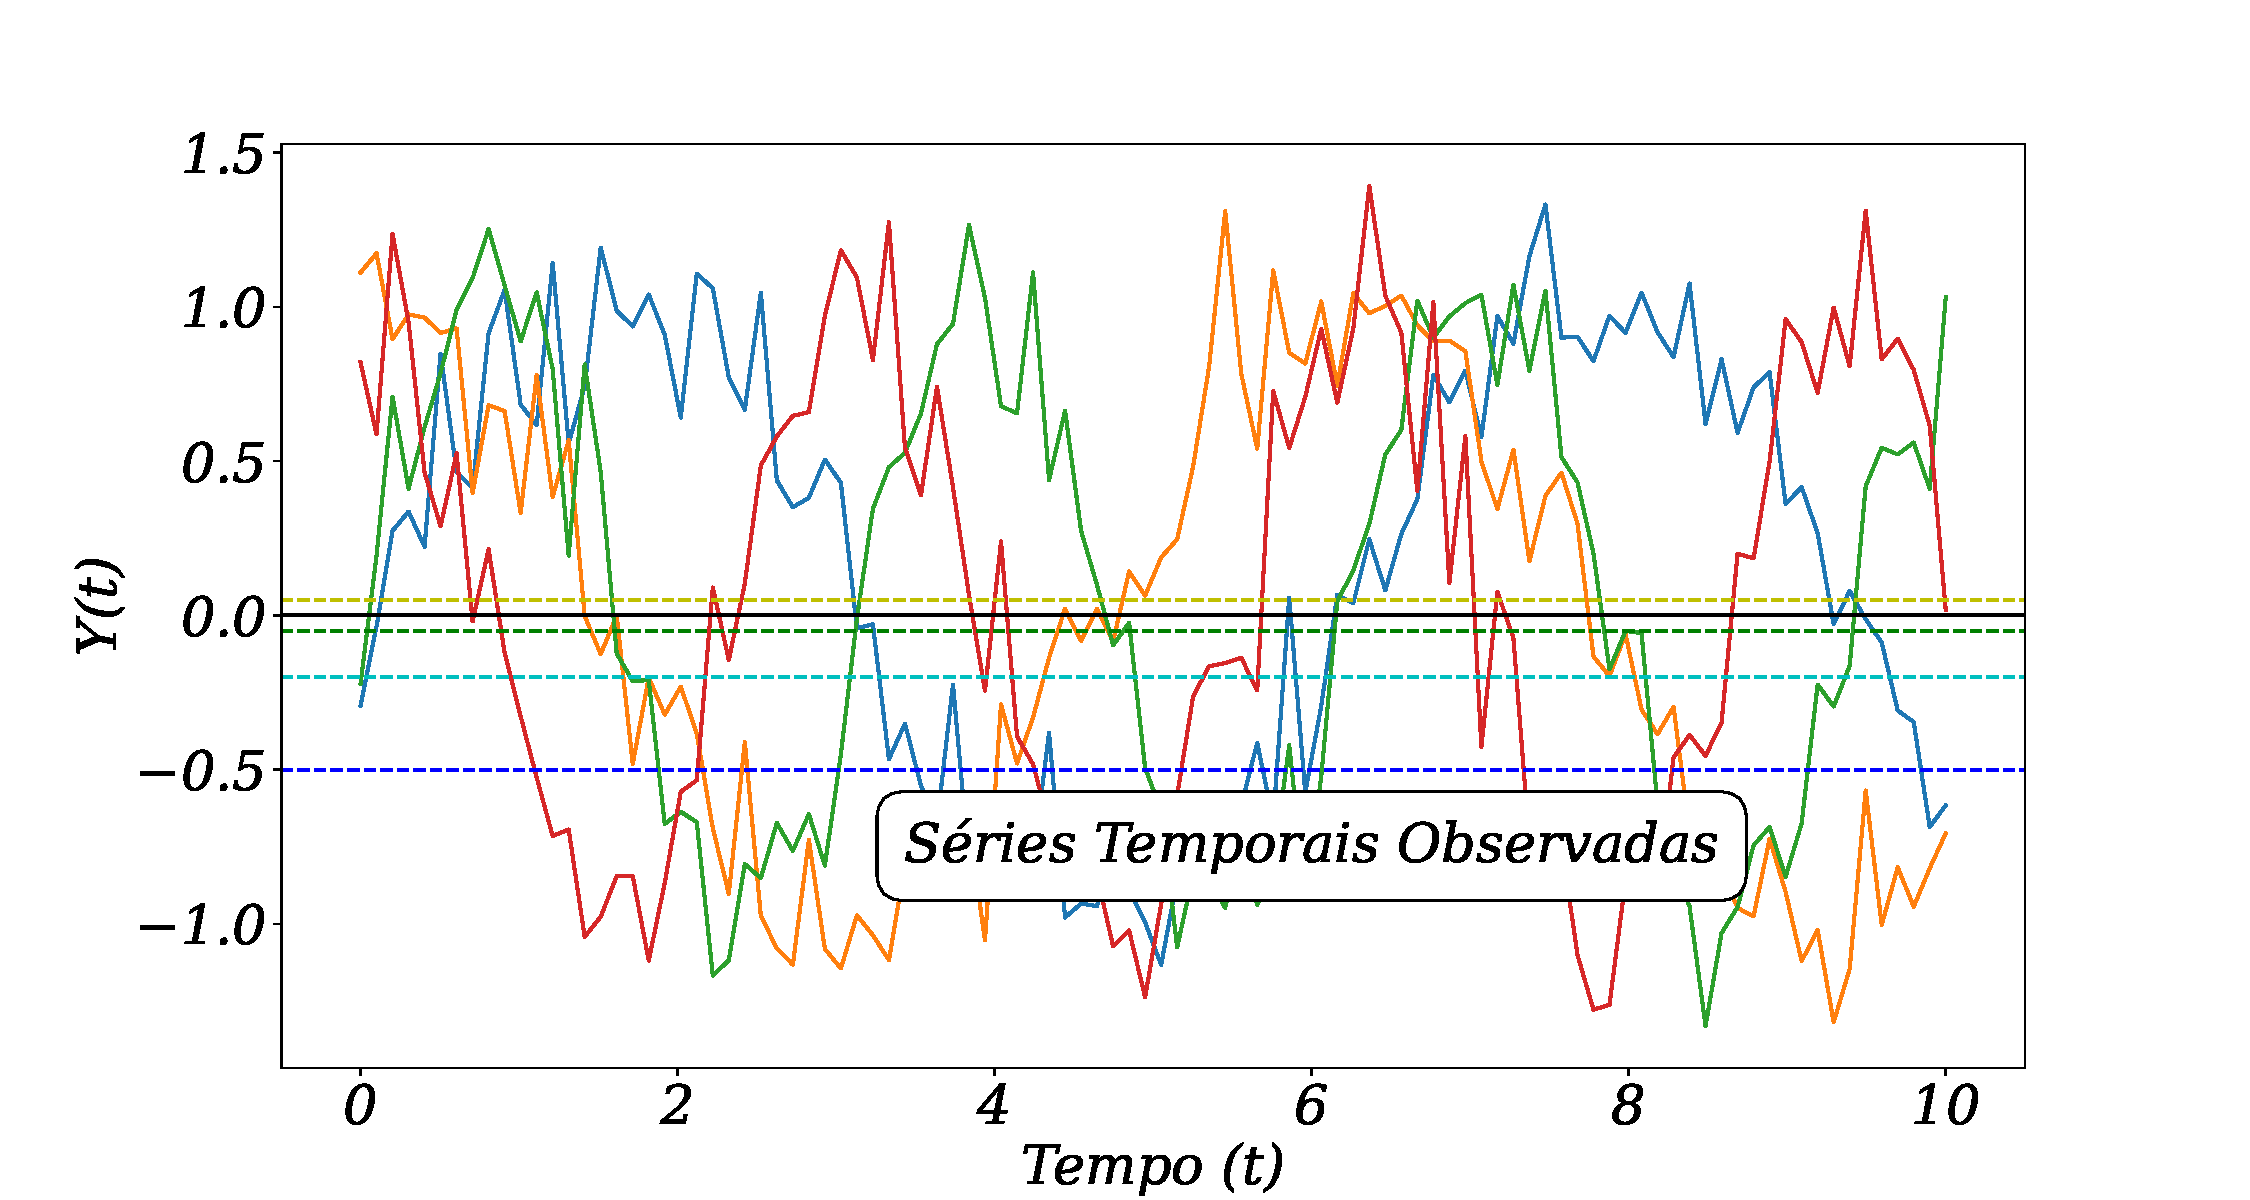
\includegraphics[width=1\linewidth]{Revisao/Figuras/serie}
	
	Fonte: \cite{pinheiro_2022}
\end{figure}

Com $Y(t)$ representando os dados fictícios e $Tempo \ (t)$ representando a linha do tempo na Figura \ref{fig:series}.

É possível pensar nisso como um conjunto de todas as trajetórias possíveis que poderiam ser observadas para uma variável.

Esta revisão sistemática da literatura aborda o tema das séries temporais, que é de grande relevância em diversas áreas, como ilustrado na Figura \ref{fig:areas}. Foi realizada uma análise das últimas seis anos para identificar as principais realizações nesse campo dentro desse curto período de tempo disponível. A seleção dos artigos foi baseada

em critérios específicos, levando em consideração a relevância dos autores, os anos de atividade, os países com maior número de publicações e as palavras-chave mais frequentes.

O objetivo dessa revisão é analisar uma literatura selecionada, porém altamente relevante. Embora a série temporal tenha como foco a análise e modelagem da dependência temporal, considerando a ordem apresentada nas bases de dados, os artigos revisados também exploram o uso de técnicas de aprendizado de máquina em aplicações relacionadas.

Embora nem todos os artigos revisados tenham uma forte relação com aprendizado de máquina, eles contribuem cientificamente para este trabalho e podem servir como base para outros pesquisadores. Essas análises fornecem uma visão básica para alguns leitores que ainda não estão familiarizados com o conceito de séries temporais ou revisões sistemáticas da literatura.
